\documentclass[sigconf]{acmart}
\usepackage[utf8]{inputenc}
\usepackage{alltt}
\usepackage{paralist}
\usepackage{enumitem}
\usepackage{url}
\usepackage{xcolor}

\usepackage{float}

\usepackage{comment}
\usepackage{todonotes}
\usepackage{latexsym}
\usepackage{amsmath}
\usepackage{multirow}
\usepackage{microtype}
\usepackage{enumitem}
\usepackage{listings}
\usepackage{makecell}

\renewcommand\floatpagefraction{.9}
\renewcommand\topfraction{.9}

\renewcommand\bottomfraction{.9}

\renewcommand\textfraction{.1}

\setcounter{totalnumber}{50}

\setcounter{topnumber}{50}

\setcounter{bottomnumber}{50}

%\addtolength{\itemsep}{-0.05in}

\addtolength{\topsep}{-0.07in}

\addtolength{\textfloatsep}{-0.05in}

\addtolength{\intextsep}{-0.05in}

\addtolength{\partopsep}{-0.03in}

%Conference
\acmConference[Devcon'18]{Graphene Devcon}{May 2018}{Shanghai, China} 
\acmYear{2018}
\copyrightyear{2018}

\setcopyright{none}

\begin{document}
\author{Customminer (@CM-STEEM)}

\title{Hertz - An Oscillating USD pegged Algorithm Based Asset}

\keywords{Bitshares, Market Pegged Assets, Algorithm Based Assets, Graphene}

\begin{abstract}
This paper will introduce Hertz which is an Algorithm Based Asset (ABA) which was created on the Bitshares Decentralized Exchange (BTS DEX). It's settlement price feed is pegged to 1 USD then predictably modified to oscillate using a sine wave with 14\% amplitude and a period of 28 days, thus introducing predictable phases of price feed appreciation and depreciation and a range of \$0.86 to \$1.14. The development process and lessons learned will also be elaborated upon so as to accelerate the implementation of future ABAs on the BTS DEX.
\end{abstract}

\maketitle
\section{Introduction}
\noindent The Bitshares Decentralized Exchange (BTS DEX) provides the ability to create Market Pegged Assets (MPAs) which are price stable cryptocurrency tokens typically pegged to external reference assets and provably backed by (typically more than 175\%) collateral in Bitshares.

Confirmation times for transactions on the BTS DEX are typically less than a couple seconds, and the BTS DEX is massively scalable\citep{bitshares_foundation_bitshares_2018}. MPAs can take full advantage of this high performance blockchain network at a small cost to the issuer (asset creation \& smartcoin setting update fees), price feed publishers (price feed publish fees) and user (transfer fees).\citep{oxarbitrage_current_2018}

\smallskip

\noindent The majority of MPAs created on the BTS DEX are backed by BTS and have external references (layer 1), however there are multiple possible layers of backing collateral for MPAs on the BTS DEX:

\smallskip

  \begin{center}
    \begin{tabular}{ | l | l | l | l |}
      \hline
      \thead{Layer} & \thead{Reference Asset} & \thead{Backing Collateral}  & \thead{Examples} \\
      \hline
      0 & Internal & BTS & N/A \\
      1 & External & BTS & \makecell{USD, Hertz \& Hero} \\
      2 & External & Layer 1 MPA & XCD  \\
      n & External & Layer n-1 MPA & N/A \\
      \hline
    \end{tabular}
  \end{center}

\medskip

MPAs are issued in a decentralized manner as they're borrowed into existence and shorted on the market without introducing counter party risk. If the shorter's backing collateral falls below the Minimum Collateral Ratio (MCR) then the shorter is force settled, forcing them to buy back their debt at market rates to then close their debt position.\citep{bitshares_foundation_dex_2018}

MPA holders can trigger a settlement at any time which exchanges their settled MPA tokens for the equivalent backing collateral from the least collateralized short position at the current settlement price rate. This means that even if a shorter has a greater collateral ratio than the MCR, they can be force settled.\citep{bitshares_foundation_dex_2018}

The settlement rate of an MPA in BTS (or an alternative backing collateral asset) is determined as the median price feed in the set of the latest published price feeds for the MPA in question.\citep{bitshares_foundation_dex_2018}

Price feeds are regularly provided by price feed publishers such as Witnesses, Committee members or manually configured private price feed publishers. You need to reach out to prospective price feed publishers directly before they will begin publishing price feeds.

Algorithm Based Assets (ABAs) are pegged to a reference asset (USD in both HERO \& Hertz case) then the reference price feed is modified using a publicly available algorithm to produce predictable effects over time. Introducing an algorithm to an MPA does not affect its backing collateral layer; both Hero and Hertz are still layer 1 MPAs, however an ABA can be created at any layer.

The primary focus of this paper is Hertz and Algorithm Based Assets on the BTS DEX.

\section{Related work}

Hero was the first ABA on the BTS DEX, its value is pegged to the USD plus 5\% appreciation per year since the FED began printing the USD back in 1913. This translates to an approximate HERO value of \$160 in 2018.\citep{hero_hero_2018}

Hero was the primary inspiration for Hertz; initially the opposite of HERO was proposed with a goal of depreciating the value x\% per year however this was economic policy was perceived as undesirable for long term holders.\citep{customminer_nemesis_2018} The Sine wave algorithm was proposed to combine the effects of HERO and its opposite theoretical ABA, resulting in predictable phases of both price feed appreciation and price feed depreciation every 28 days forever.

There are no examples of assets which have implemented a similar algorithm to oscillate its value like Hertz in neither the FIAT nor Cryptocurrency markets, so the concept is unique and highly experimental. There are however over the counter financial derivatives such as variance and volatility swaps which may share similar trading behaviour as Hertz.

Unlike variance and volatility swaps, there is no expiration on shorted positions aside from force settlement (either due to under collateralization or being the least collateralized short position upon Hertz asset settlement). The shorter's ability to close their position depends entirely on them buying back their debt from the open market.

Unlike established volatility/variance products like the Volatility Index (VIX) and the DJIA Volatility Index (VXD), Bitshares DEX market participants can trade Hertz directly with one another with no middlemen involved in the process. It may be worth implementing such volatility/variance products as MPAs on the BTS DEX in the future, however such proposals are out of scope from this paper.

\section{Hertz Overview}

Hertz is an Algorithm Based Asset (layer 1 MPA) which is pegged to the current USD value (in BTS) and modified to oscillate using a sine wave algorithm.\citep{customminer_hertz_2018} This section will provide more info on what Hertz is, how it was created and how you could create an alternative implementation if interested.

\subsection{Price feed scripts}

\noindent Many price feed publishers have different price feed script solution preferences thus there are three open source multi-asset price feed script repos you'll need to provide implementations of your ABA for in order to enable the majority of BTS witnesses to publish price feeds. 

The more price feed scripts you integrate your algorithm into, the more likely you are to recruit a greater quantity of price feed publishers for your ABA on the BTS DEX. Likewise, if your ABA price feed publishers utilize multiple price feed scripts the greater the redundancy (you don't want one glitch stopping all price feeds).

It's worthwhile creating a reference price feed script which doesn't involve the existing price feed script repos, so that if there are delays in integration you'll have a backup option for witnesses to use.

\smallskip

\noindent Current community created price feed scripts:
\begin{enumerate}[wide, labelwidth=!, labelindent=0pt]
\item Wackou's BTS\_Tools (supports Hertz)\citep{wackou_wackous_2018}
\item Xeroc's bitshares-pricefeed \citep{xeroc_xerocs_2018} 
\item pch957's btsprice \citep{pch957_pch957s_2018}
\item python-bitshares based reference price feed scripts\citep{customminer_reference_2018}
\end{enumerate}

\subsection{Hertz algorithm}

\noindent Hertz is primarily implemented in Python across four different price feed scripts (as mentioned above). It implements a sine wave to provide a predictable oscillation to the settlement price over the course of 28 days. 

By implementing an amplitude of 14\% a settlement price range of \$0.86 to \$1.14 is achieved. Note that the settlement price and market trading rates are not the same, it's likely that market participants will trade above/below the settlement price depending on the ongoing oscillation.

Wednesdays were chosen as the primary milestone day as this is mid working week for the UTC timezone.

\bigskip

\noindent 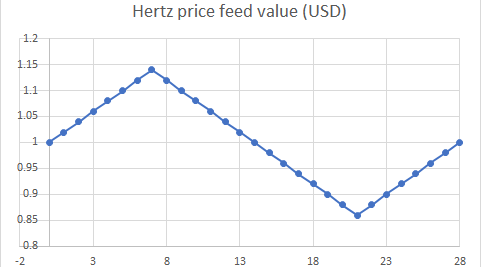
\includegraphics[width=\columnwidth]{hertz_chart.png}

\bigskip

\noindent The above image shows the Hertz settlement price in USD across the 28 day period.

\bigskip

\noindent The following Hertz Python pseudocode will briefly demonstrate how the Hertz algorithm is implemented.

\lstset{language=Python,
		caption=Hertz Python Pseudocode,
    	label={Hertz Python Pseudocode},
    	breaklines=true}

\begin{lstlisting}[frame=single]
from math import pi, sin

period = 2419200 # 28 days in seconds
hz_phase = 0.908056 # Time offset
amplitude = 0.14 # 14%

# Bitshares 2.0 genesis block timestamp:
ref_time = "2015-10-13T14:12:24+00:00" 

time_diff = timestamp - (ref_time + phase)

hz_now = ((time_diff/period) % 1) * period

sin_calc = sin(hz_now * ((2*pi)/period))

hertz_value = 1 + (amplitude * sin_calc)
\end{lstlisting}

\bigskip

Static variables are referenced for the amplitude, reference timestamp, period, phase and reference asset. Only the current time and current 'BTS:USD' rate (not included in code for simplicity) are dynamic, and only the 'BTS:USD' rate is an unknown factor for all participants.

Simply put, we estimate the current point of the sine wave and apply either a positive or negative value to the reference asset value through addition, resulting in a settlement price range of \$0.86 to \$1.14.

Given the MIT licensed open source licensing of the Hertz price feed scripts, it's possible for anyone to create a new ABA with alternative static variables

It's highly advisable to research the impact of changing the variables and finalizing your selection prior to activation on the BTS DEX, as coordinating the modification of these static variables could prove difficult.

\bigskip

\noindent Modifiable static variables:
\begin{enumerate}[wide, labelwidth=!, labelindent=0pt]
\item Reference asset (USD, CNY, EUR..).
\item Amplitude (7\%, 14\%, 50\%..).
\item Period (7 days, 14 days, 30 days..).
\item Wave algorithm (Sine, Cos, Combination..).
\item Phase (Offset reference/genesis timestamp to a specific day of the week).
\item Preferred timezone (Default: UTC).
\item Reference timestamp (Default: BTS2.0 genesis timestamp).
\end{enumerate}

\noindent Smartcoin settings:

\begin{enumerate}[wide, labelwidth=!, labelindent=0pt]
\item Minimum collateral ratio: 200\%
\item Max force settle volume: 5\%
\item Percent offset of forced settlements: 1\%
\item Force settlement delay: 1440 mins
\item Short backing asset: BTS
\end{enumerate}

\subsection{Surrendered Smartcoin flags/permissions}

Unlike many of the current Bitshares committee controlled smartcoins (such as bitUSD), the following flags were permanently disabled in order to improve the decentralization of Hertz.

\smallskip

\begin{enumerate}[wide, labelwidth=!, labelindent=0pt]
\item "Require holders to be white-listed":	There will never be a white-list for holders.
\item "Issuer may transfer asset back to himself": The issuer can never transfer the asset back to themselves. 
\item "Issuer must approve all transfers": Transfers will never require approval.
\item "Disable confidential transactions": Confidential transactions (whenever implemented) will always be allowed. 
\end{enumerate}

You shouldn't be concerned that assets currently controlled by the committee could be manipulated through the above permissions, as committee members are elected by BTS holders and any such actions are highly transparent on the blockchain. The removal of these permissions simply makes such a small risk entirely impossible to improve user confidence.

\section{Predicted effects of Hertz}

Hertz is a highly experimental smartcoin on the BTS DEX, all code is MIT licensed and price feeds are provided in a decentralized manner. This paper does not constitute financial advice. Do your research, consult financial advisors and then acknowledge the risks prior to trading Hertz.

Hertz can experience unpredictable contamination of volatility through USD and BTS value exposure as well as through unpredictable market trading behaviour caused by the sine wave based price feed oscillation.

With that disclaimer out of the way, this section will detail some of the theorized effects of the Hertz ABA.

\subsection{Price feed appreciation}

The price feed value appreciates from \$0.86 on day 21 (previous cycle) to \$1.14 on day 7 (next cycle); this price feed appreciation benefits the Hertz holder at the expense of the shorter (their collateral ratio decreases), unless the value of BTS increases more than 28\% in this time frame.

\subsection{Price feed depreciation}

The price feed value depreciates from \$1.14 on day 7 to \$0.86 by day 21; this price feed depreciation benefits the shorter (through temporary debt destruction \& subsequent collateral ratio increase) unless the value of BTS decreases in value more than 28\% in this time frame.

\subsection{Peak settlement price}

Day 7 of 28 is the peak settlement price after which the price feeds will begin to depreciate.

\begin{enumerate}[wide, labelwidth=!, labelindent=0pt]
\item Shorters aiming to maximize benefits from price feed depreciation may produce peak selling pressure.
\item Holders producing peak settle pressure as they realize price feed appreciation gains from past hertz cycles.
\item Less buy pressure, as holders will have to wait 28 days (a full cycle) before their Hertz tokens return to this rate, and they will not benefit from price feed appreciation.
\item The potential shorter sell wall may provide sell liquidity not currently possible with other MPAs without having an impact on the core BTS trading rate.
\end{enumerate}

\subsection{Trough settlement price}

Day 21 of 28 is the trough feed value, Highest theoretical buy pressure however Lowest predicted sell and settle pressure!

\begin{enumerate}[wide, labelwidth=!, labelindent=0pt]
\item Shorters selling Hertz during the trough face impending price feed appreciation then settlement at the peak value. This may result in a lack of sell liquidity during the trough which affects shorters ability to buy back debt at trough rates.
\item Shorters aiming to buy BTS during the trough to settle their debt and realize any potential debt destruction will be a likely source of predictable buy pressure.
\item Holders aiming to buy in the trough to then settle at the peak will additionally be a likely source of predictable buy pressure.
\item Combined shorter and holder potential buy wall may provide shorters larger trading opportunities than currently possible with traditional MPAs (without impacting BTS core price).
\end{enumerate}

\subsection{Long term holders}
It's highly likely that some Hertz holders will hold their tokens long term, especially if they were to buy at the peak and have to wait until subsequent peaks to settle.

It's less likely that those who buy in a trough will hold through peaks, unless BTS is more volatile than Hertz and settling would be detrimental.

It's possible that due to long term holding behaviour, that there may be insufficient liquidity for the shorter to buy back their debt and thus be locked into holding debt without an exit. This is potentially only a risk during the initial startup cycles until sufficient liquidity has developed throughout all phases of the hertz cycle.

\section{Future work}

Several future goals are the following:

\begin{enumerate}[wide, labelwidth=!, labelindent=0pt]
\item Full price feed script ocverage - There is an open bounty for the implementation of Hertz in pch957's btsprice repo, afterwhich we will have achieved 100\% BTS price feed script coverage.
\item Maximizing the quantity of Hertz price feed publishers, preferably more than 20.
\item Creating alternative Hertz ABAs with different static variables.
\item Implementing an alternative calendar system than the 28 day calendar, accounting for leap years and different sized months. Only for an alternative Hertz ABA.
\item Experiment with layer 0, 2 and n backing collateral ABAs.
\item Once fully operational, petition the committee to accept ownership of the Hertz ABA, so as to further improve decentralization.
\item Potentially creating volatility/variance product MPAs, given their popularity in the FIAT markets.
\end{enumerate}

\newpage

\section{Lessons learned}

This section will quickly summarize the lessons learned during the implementation of Hertz over the course of the last year.

\smallskip

\begin{enumerate}[wide, labelwidth=!, labelindent=0pt]
\item Communication with price feed publishers is key. You need to reach out to price feed publishers directly and help troubleshoot any issues they encounter when running your price feed scripts. It can take several months to establish a large set of price feed publishers whom are all publishing accurate price feeds.
\item You must thoroughly test the price feed scripts prior to requesting price feed publishers use them, this will save you time troubleshooting and will reduce potentially frustrating price feed publishers. 
\item Integrating your algorithm into existing price feed scripts can take several weeks per pull request since the repository owners are very busy individuals.
\item Hertz static variables must be thoroughly considered prior to integration into price feed scripts. Initially the amplitude was 50\% before being reduced to 33\% then finally 14\%; be careful not to create too volatile an ABA! Use the spreadsheet hertz calculator to gauge static variable impact upon collateral ratios throughout a full cycle.
\item Whilst using the testnet for testing your ABA is free, there are complexities (TEST doesn't have a value, there's no reference bitUSD asset) which can impede testing ABAs on testnet. \item You can easily test price feed publishing in production without any problems if you set the minimum price feed publisher quantity to a value far greater than the current price feed publisher count.
\end{enumerate}

\section{Conclusion}

It's possible to introduce predictable velocity to an MPA on the BTS DEX by applying a sine wave based oscillation to an USD pegged MPA resulting in phases of price feed appreciation and depreciation; such effects introduced by Hertz are highly unique and require further observation once active on the BTS DEX.

Algorithm Based Assets like Hertz are cheap to implement, decentralized, highly collateralized and free from counter-party risk. Hopefully this paper will aid the creators of subsequent Hertz derivatives by encouraging a more streamlined development experience \& Algorithm Based Assets as a result will gain more attention within BTS and the greater cryptocurrency community in the future.

\bibliographystyle{plainnat}
\bibliography{Zotero}


\end{document}